\section*{Problem 3: Random Kitchen Sinks and a one-hidden-layer MLP}

\paragraph{(a) Training data.} The supplied splits contain 600 training observations, 200 validation observations, and 200 unlabeled test inputs. The colored scatter plot on the next page shows a smooth response: a broad low region near $(x_1,x_2)=(-1.5,0)$, increasing values toward $|x_2|=3$, and a curved variation along $x_1$.

\paragraph{(b) Random Kitchen Sinks.} I draw $h=D/2$ Gaussian projections $w_j\sim N(0,I/\sigma^2)$ and phases $b_j\sim U[0,2\pi]$. The features are
\[
\phi(x)=\frac{1}{\sqrt h}\big(\sin(w_1^Tx+b_1),\cos(w_1^Tx+b_1),\ldots,
\sin(w_h^Tx+b_h),\cos(w_h^Tx+b_h)\big)^T.
\]
The factor $1/\sqrt h$ keeps the overall feature scale comparable across widths. I fit an unpenalized intercept and ridge coefficients by minimizing
\[
\sum_{i\in\mathrm{train}}\big(y_i-a-\beta^T\phi(x_i)\big)^2+\lambda\|\beta\|_2^2.
\]
Only $D$ varies; $\sigma=1$ and $\lambda=10^{-3}$ remain fixed. The validation minimum occurs at $D=50$, or $h=25$. Increasing $D$ further lowers training error but slightly increases validation error, consistent with overfitting.

\paragraph{(c) One-hidden-layer MLP.} I use a $2\to m\to1$ network with a tanh hidden activation and a linear output. Inputs and the target are standardized using training-set statistics; predictions are returned to the original target scale. I vary only the hidden width $m$. All models use Adam with learning rate $0.01$, batch size 600, 4,000 epochs, and weight decay $10^{-5}$. Initialization uses seed 42. The lowest validation MSE occurs at $m=256$, although $m=16$ is almost tied. Width therefore does not have a simple monotone relationship with validation performance in this run.

\begin{center}
\begin{minipage}[t]{0.47\textwidth}
\centering
\textbf{RKS sweep}\\[5pt]
\begin{tabular}{rrr}
\toprule
$D$ & Train MSE & Val. MSE\\
\midrule
10 & 0.778920 & 0.710045\\
20 & 0.058264 & 0.056286\\
50 & 0.032399 & \textbf{0.037138}\\
100 & 0.031681 & 0.037500\\
200 & 0.030800 & 0.038400\\
400 & 0.030247 & 0.038517\\
800 & 0.029581 & 0.040825\\
1200 & 0.029477 & 0.041498\\
\bottomrule
\end{tabular}
\end{minipage}\hfill
\begin{minipage}[t]{0.47\textwidth}
\centering
\textbf{MLP sweep}\\[5pt]
\begin{tabular}{rrr}
\toprule
$m$ & Train MSE & Val. MSE\\
\midrule
8 & 0.033222 & 0.036675\\
16 & 0.032935 & 0.036101\\
32 & 0.031560 & 0.037585\\
64 & 0.031941 & 0.037584\\
128 & 0.032663 & 0.036467\\
256 & 0.032829 & \textbf{0.036007}\\
\bottomrule
\end{tabular}
\end{minipage}
\end{center}

\paragraph{(d) Final fits and predictions.} After selection, I refit both models on the training split using their selected hyperparameters and the same seed. Validation labels remain outside fitting. RKS has validation MSE $0.037138$ and MLP has $0.036007$, a roughly $3.0\%$ lower MSE for the MLP. Its hidden features adapt to the response, whereas the RKS features are fixed random draws. Both fit this smooth function well; the small difference on one validation split does not establish a general advantage.

The output files are \texttt{rks\_test\_predictions.csv} and \texttt{mlp\_test\_predictions.csv}. Each contains the header \texttt{prediction} followed by 200 predictions in the original test-row order. Test MSE cannot be computed because those labels are withheld.

\newpage
\begin{figure}[H]
\centering
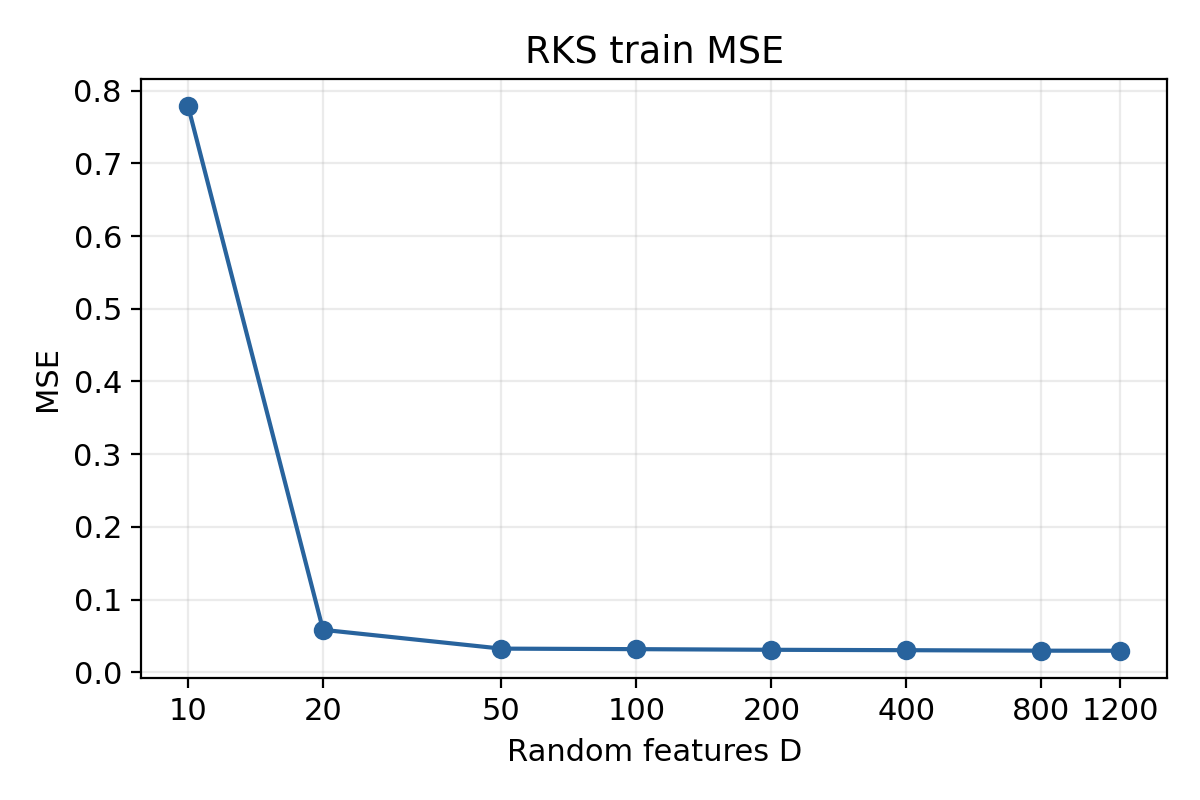
\includegraphics[width=0.48\textwidth]{images/problem3/rks_train_mse.png}\hfill
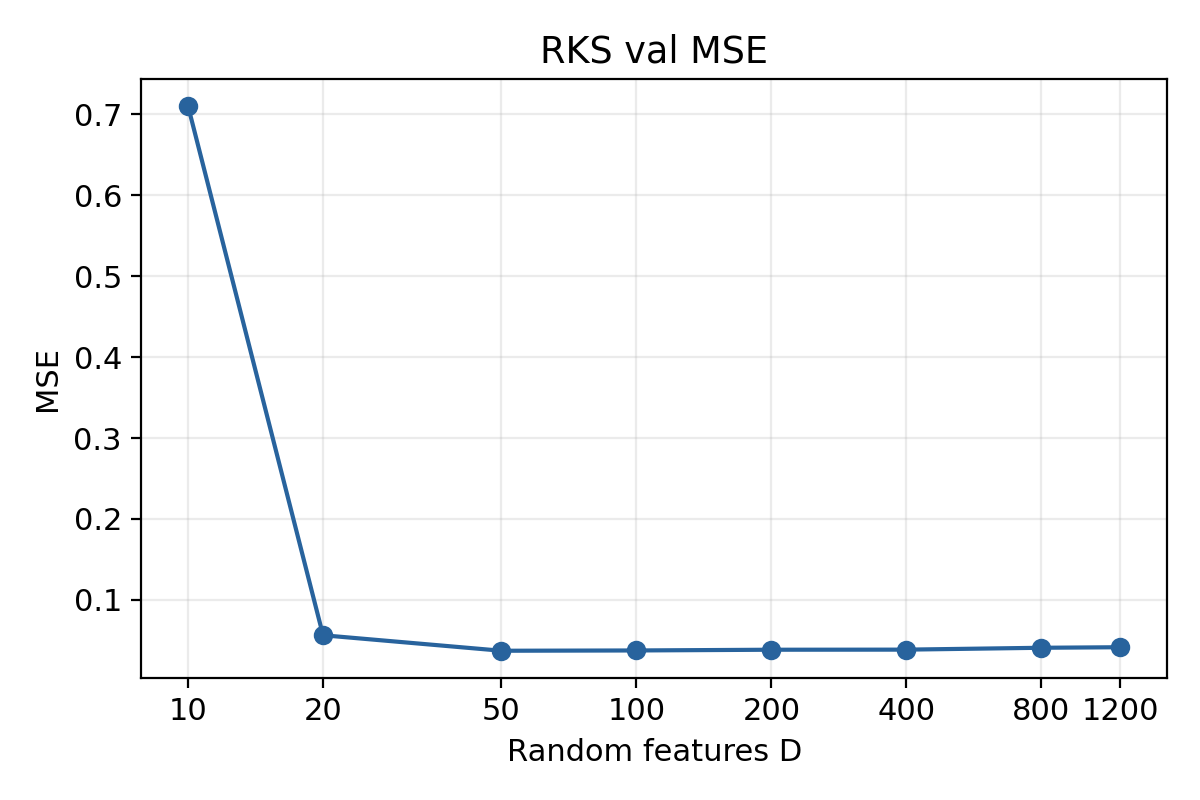
\includegraphics[width=0.48\textwidth]{images/problem3/rks_val_mse.png}\\[3pt]
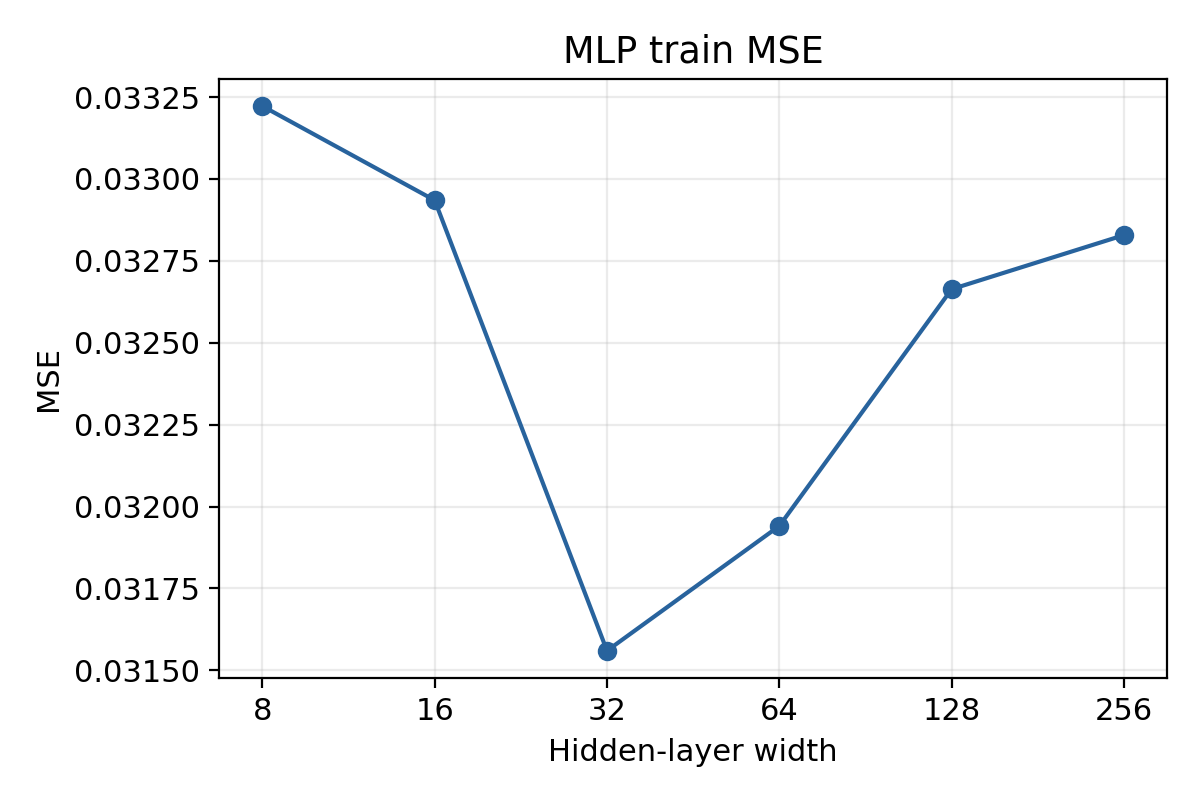
\includegraphics[width=0.48\textwidth]{images/problem3/mlp_train_mse.png}\hfill
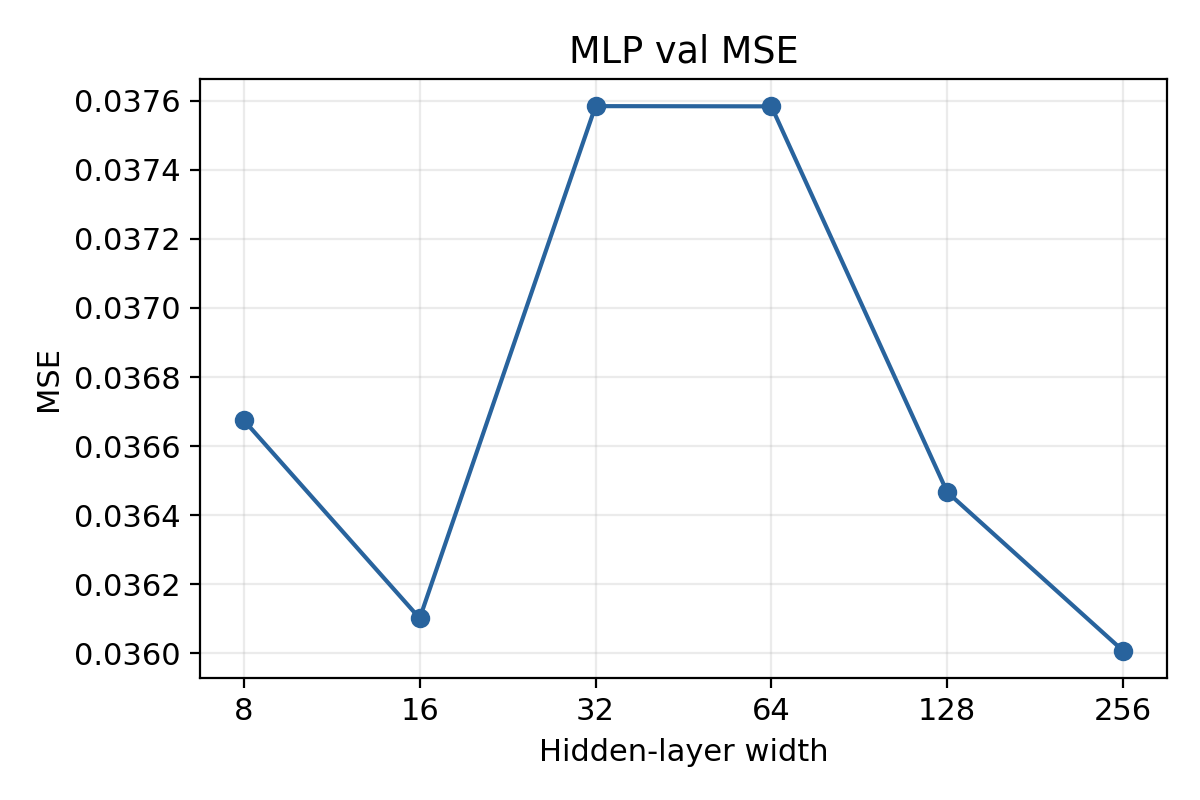
\includegraphics[width=0.48\textwidth]{images/problem3/mlp_val_mse.png}
\caption{Training and validation MSE across the two hyperparameter sweeps.}
\end{figure}
\begin{figure}[H]
\centering
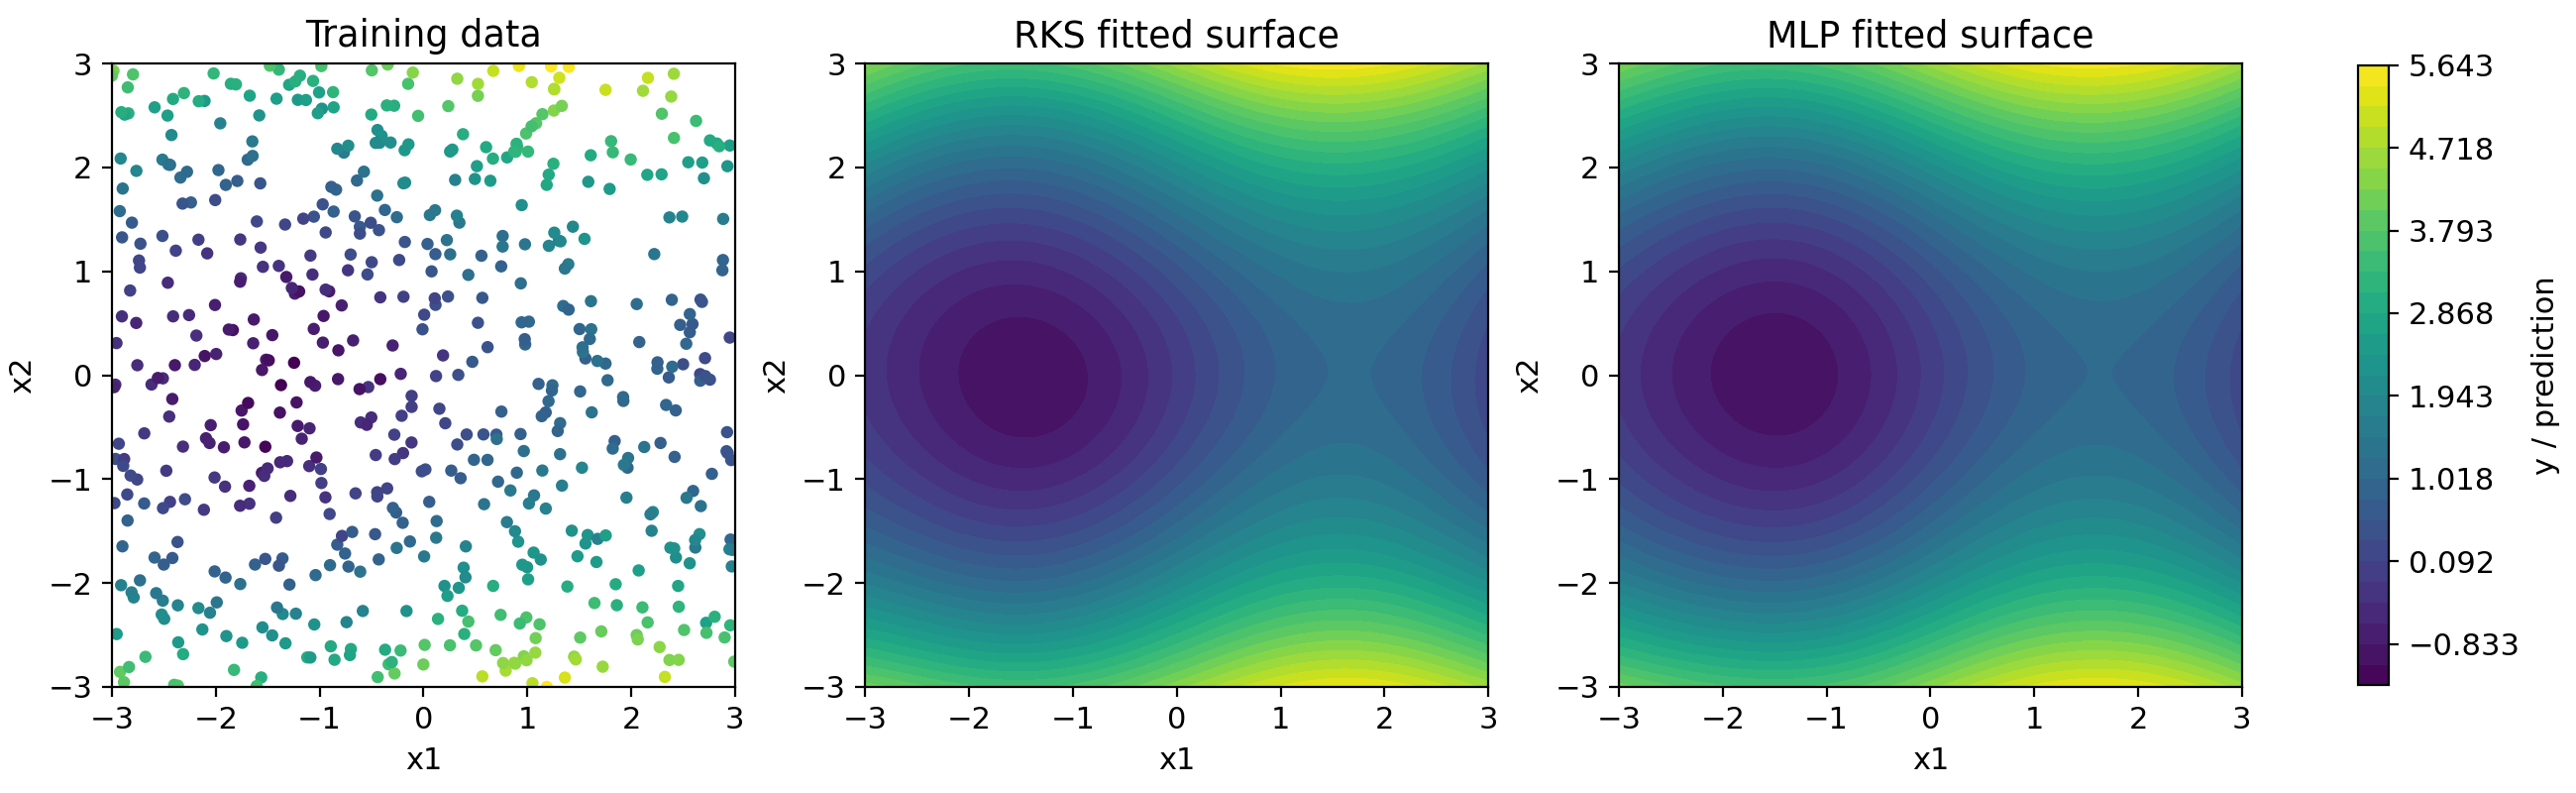
\includegraphics[width=\textwidth]{images/problem3/surface_comparison.png}
\caption{Training observations and the selected fitted functions over $[-3,3]^2$, using a common color scale.}
\end{figure}
Both surfaces recover the broad trough, high values near the top and bottom boundaries, and the curved pattern across $x_1$. Neither follows the pointwise noise. The RKS surface is slightly more rounded near the left boundary, while the MLP has learned a similar shape with adaptive hidden features. These similarities agree with their close validation errors.
